\documentclass{article}
\usepackage[left=3cm,right=3cm,top=3cm,bottom=3cm]{geometry}
\usepackage{amsmath,amssymb,amsthm,pgfplots,tikz}
\usepackage{color}
%\setlength{\parindent}{0mm}

\newcommand{\TODO}[1]{\textcolor{red}{TODO: #1}}

\begin{document}
\title{Graduate Algebra I: Homework 3}
\author{Li Ling Ko\\ lko@nd.edu}
\date{\today}
\maketitle

\begin{enumerate}
  \item
    \begin{enumerate}
      \item Consider $A=\{(1,2,3,4)\}\subset S_4$. Compute the centralizer
        and the normalizer of $A$ in $S_4$.

        \begin{proof}
          Since $A$ has a single element, by chasing definitions, its
          normalizer is the same as its centralizer.
          The elements of $S_4$ are either the identity, a 2-cycle, a
          3-cycle, two disjoint 2-cycles, or a 4-cycle. We check which of
          these elements $(1,2,3,4)$ commutes with. We observe that if a
          given element $g$ commutes with another element $h$, then $g$
          would commute with the subgroup generated by $h$, since $gh=hg$
          implies from induction on $r$ that $gh^r=h^rg$. Hence we do not
          need to check for commutativity with an element in the cyclic
          subgroup of another element which was found to commute with
          $(1,2,3,4)$. We also use symmetrical arguments to decrease the
          number of times we need to check for commutativity. \\

          Clearly the identity commutes with $(1,2,3,4)$. As for the
          2-cycles, we check that $(1,2)$ does not commute with
          $(1,2,3,4)$, so by symmetry, neither should $(2,3)$, $(3,4)$, or
          $(4,1)$. Also, we check that $(1,3)$ does not commute with
          $(1,2,3,4)$, so by symmetry, neither should $(2,4)$. Next, we
          check for commutativity with the 3-cycles. $(1,2,3,4)$ does not
          commute with $(1,2,3)$, and since $(1,2,3)$ is contained in the
          group generated by $(1,3,2)$, $(1,2,3,4)$ would not commute with
          $(1,3,2)$ either. Also by symmetry, $(1,2,3,4)$ should not
          commute with $(2,3,4)$ if it did not commute with $(1,2,3)$,
          which means $(1,2,3,4)$ would not commute with $(2,4,3)$.
          Finally, $(1,2,3,4)$ does not commute with $(1,2,4)$, so it will
          not commute with $(1,4,2)$. So $(1,2,3,4)$ does not commute with
          any 2-cycles or 3-cycles. \\

          Next, we check commutativity with the 4-cycles. Clearly
          $(1,2,3,4)$ commutes with itself and hence with any 4-cycle in
          its cyclic subgroup. We check that $(1,2,3,4)$ does not commute
          with $(1,2,4,3)$, $(1,3,4,2)$, $(1,3,2,4)$, $(1,4,2,3)$, or
          $(1,4,3,2)$. Any other 4-cycle not in $\langle A\rangle$
          generates a cyclic subgroup that contains one of these
          non-commutating elements, so the only 4-cycles that commute with
          $(1,2,3,4)$ are those in its cyclic subgroup. Finally, we check
          for commutativity with the disjoint 2-cycles. We check that
          $(1,2,3,4)$ does not commute with $(1,2)(3,4)$, $(1,3)(2,4)$,
          or $(1,4)(2,3)$, which are all the possible disjoint 2-cycles. We
          conclude that the centralizer of $A$, which is also its
          normalizer, is the its cyclic subgroup, which is
          $\langle(1,2,3,4)\rangle$. \\
        \end{proof}

      \item Consider $H=\langle(1,2,3,4)\rangle\subset S_4$. Compute the
        centralizer and the normalizer of $H$ in $S_4$.

        \begin{proof}
          We first find the centralizer. By the definition of centralizer,
          we have $C_G(\langle g\rangle)\subseteq C_G(\{g\})$ for any
          element $g\in G$. Also, if $h$ commutes with $g$, then $h$ will
          also commute with $g^r$, since $gh^r=h^rg$ by induction on $r$.
          Hence $C_G(\langle g\rangle)\supseteq C_G(\{g\})$, which implies
          that $C_G(\langle g\rangle)=C_G(\{g\})$. Therefore, the
          centralizer of $H$ is the centralizer of $A$, which we have
          computed earlier to equal to $H$ itself. \\

          Now we find the normalizer of $H$. By the definition of a
          normalizer, we have $N_G(\langle g\rangle)\supseteq N_G(\{g\})$
          for any element $g\in G$, hence $N(H)$ must contain at least
          $N(A)$, which we have found to be the cyclic group generated by
          $(1,2,3,4)$. We check which other elements of $S_4$ should be
          contained in $N(H)$. Let $a$ denote $(1,2,3,4)$. Then
          $gH=\{g,ga,ga^2,ga^3\}$, and $Hg=\{g,ag,a^2g,a^3g\}$. For $gH$
          to equal $Hg$, we need to find a surjection between the two
          sets, so $ga$ should be mapped to either $g$, $ag$, $a^2g$, or
          $a^3g$. If $ga$ is mapped to $g$, we get $a=1$, a
          contradiction. If $ga$ is mapped to $ag$, then $g$ would be in
          $C(H)$, which we have computed earlier to equal $H$. If $ga$ is
          mapped to $a^2g$, then $ga^2$ will be mapped to $a^2ga=a^4g=g$,
          which is a contradiction since the inverse image of $g$ should
          only be $g$. Finally, if $ga$ is mapped to $a^3g$, then we will
          get a bijection between $gH$ and $Hg$ which maps $g$ to $g$,
          $ga$ to $a^3g$, $ga^2$ to $a^2g$, and $ga^3$ to $ag$. Hence it
          remains to find all $g\in G$ such that $gag^{-1}$ equals $a^3$.
          \\

          Once we find an element $g\in G$ satisfying $gag^{-1}=a^3$, then
          we know all elements in the group generated by $a$ and $g$ must
          also be in the normalizer, since normalizers are subgroups. This
          reduces the number of checks we need to perform. \\

          We first check which 2-cycles will satisfy the criteria
          $gag^{-1}=a^3=(4,1,2,3)$. We find that $(1,3)$ satisfies the
          criteria. Therefore, from the above observation, we know that
          $\langle(1,3),(1,2,3,4)\rangle$ is in $N(H)$. We check that
          $\langle(1,3),(1,2,3,4)\rangle$ has eight distinct elements, each
          with order either 1, 2, or 4. Since the order of subgroups must
          divide the order of the group, the order of $N(H)$ must be a
          multiple of 8 and also a divisor of $|S_4|=24$, which means the
          order of $N(H)$ can only be 8 or 24, further implying that $N(H)$
          can only be $\langle(1,3),(1,2,3,4)\rangle$ or the whole of
          $S_4$. We check that $(1,2)$ does not satisfy
          $gag^{-1}=a^3=(4,1,2,3)$ and hence cannot be in $N(H)$, and so
          $N(H)=\langle(1,3),(1,2,3,4)\rangle$.
        \end{proof}
    \end{enumerate}

  \item Again consider $H=\langle(1,2,3,4)\rangle\leq S_4$.
    \begin{enumerate}
      \item Calculate the left coset $(1,2)H$ in $S_4$.
        \begin{proof}
          The table below summarizes the calculations.
          \begin{center}
            \begin{tabular}{|l|l|}
              \hline
              $h\in H$      & $(1,2)h$    \\ \hline\hline
              $e$           & $(1,2)$     \\ \hline
              $(1,2,3,4)$   & $(2,3,4)$   \\ \hline
              $(1,2,3,4)^2$ & $(1,3,2,4)$ \\ \hline
              $(1,2,3,4)^3$ & $(4,3,1)$   \\ \hline
            \end{tabular}
          \end{center}
        \end{proof}

      \item Calculate the right coset $H(1,2)$ in $S_4$.
        \begin{proof}
          The table below summarizes the calculations.
          \begin{center}
            \begin{tabular}{|l|l|}
              \hline
              $h\in H$      & $h(1,2)$    \\ \hline\hline
              $e$           & $(1,2)$     \\ \hline
              $(1,2,3,4)$   & $(1,3,4)$   \\ \hline
              $(1,2,3,4)^2$ & $(1,4,2,3)$ \\ \hline
              $(1,2,3,4)^3$ & $(2,4,3)$   \\ \hline
            \end{tabular}
          \end{center}
        \end{proof}

      \item Is $H$ normal in $G$?
        \begin{proof}
          $H$ is not normal in $G$. A subgroup is normal in a group if and
          only if the normalizer of the subgroup with respect to the group
          is the whole group. We have shown in question 1b that the
          normalizer of $H$ is not the whole group $S_4$, so $H$ cannot be
          normal in $S_4$.
        \end{proof}
    \end{enumerate}

  \item Let $H\subset S_4$ consist of all those permutations $\sigma$ such
    that $\sigma(4)=4$.

    \begin{enumerate}
      \item Prove that $H$ is a subgroup of $S_4$, and show that it is
        isomorphic to $S_3$.
        \begin{proof}
          Every permutation that fixes the last element is a permutation of
          the first three elements, and every permutation of only three
          elements can be considered a permutation of four elements but
          with the last element fixed. Hence the identity map from $S_3$
          to $S_4$ is a natural embedding with image $H$. This map is a
          homomorphism, so the image $H$ must be a subgroup of $S_4$ since
          the image of homomorphisms are subgroups of the codomain. Hence,
          $S_3$ is isomorphic to $H$.
        \end{proof}

      \item Is $H$ normal in $S_4$?
        \begin{proof}
          No. Consider the element $g=(1,4)(1,2)(1,4)^{-1}$. Since
          $(1,2)$ is contained in $H$, $g$ should also be contained in $H$
          if $H$ is normal. However, $g=(2,4)\not\in H$.
        \end{proof}
    \end{enumerate}

  \item Prove that if $H$ is a subgroup of $G$ of index 2, then $H$ is
    normal in $G$.
    \begin{proof}
      Let $g\in G\setminus H$, and consider the left coset $gH$ in $G$.
      Since left actions partition $G$ into equivalence classes of equal
      sizes, and the size of $gH$ must be the size of $eH=H$, which is half
      the size of $G$. Also, by the equivalence relation, $gH$ and $eH=H$
      must be disjoint since $g$ is not contained in $H$, which implies
      that $gH=G\setminus H$. Similarly for the right coset $Hg$ in $G$, we
      get $Hg=G\setminus H$. So $gH=Hg$ for any $g\in G\setminus H$. Also,
      for $g\in H$, clearly we have $gH=Hg$, hence $gH=Hg$ for all $g\in
      G$, which means $H$ is a normal subgroup of $G$.
    \end{proof}

  \item Section 2.2
    \begin{enumerate}
      \item Question 9: For any subgroup $H$ of $G$ and any nonempty subset
        $A$ of $G$ define $N_H(A)$ to be the set $\{h\in H\,|\;
        hAh^{-1}=A\}$. Show that $N_H(A)=N_G(A)\cap H$ and deduce that
        $N_H(A)$ is a subgroup of $H$.

        \begin{proof}
          The equivalence relation is true by chasing definitions: If $h\in
          N_H(A)$, then it must be contained in $H$, and also contained in
          the normalizer of $A$ with respect to $G$; if $h$ is contained in
          $H$ and is also contained in the normalizer of $A$ with respect
          to $G$, then $h$ must be in $N_H(A)$. \\

          We first show that the intersection of subgroups $H_1$ and $H_2$
          is a subgroup of the both subgroups: $H_1\cap H_2$ is non-empty
          since it contains $e$.  Also, if $a,b\in H_1\cap H_2$, then
          $ab^{-1}\in H_1,H_2$ since $H_1$ and $H_2$ are subgroups,
          implying that $ab^{-1}\in H_1\cap H_2$, which concludes our proof
          that $H_1\cap H_2$ is a subgroup of $H_1$ and $H_2$. So since
          both $H$ and $N_G(A)$ are subgroups of $G$, their intersection
          must be a subgroup of $H$, as we are required to show.
        \end{proof}

      \item Question 10: Let $H$ be a subgroup of order 2 in $G$. Show that
        $N_G(H)=C_G(H)$. Deduce that if $N_G(H)=G$ then $H\leq Z(G)$.

        \begin{proof}
          By definition of normalizers and centralizers, normalizers
          should contain the centralizers. We prove the opposite inclusion
          by chasing definitions. A subgroup $H$ of order 2 must be
          composed of an element $h$ of order 2 and the identity $e$. Hence
          $n\in N_G(H)$ is equivalent to
          $\{n,nh\}=n\{e,h\}=\{e,h\}n=\{n,hn\}$, which is equivalent to
          $nh=hn$, which is equivalent to $n$ being contained in $N_C(H)$.
          Hence $N_G(H)$ is also a subset of $N_C(H)$, so both groups are
          equivalent. \\

          From the above argument, $n\in N_G(H)$ for a subgroup $H=\{e,h\}$
          of order 2 is equivalent to $nh=hn$. So $N_G(H)=G$ implies that
          $h$ commutes with all elements of $G$, which means that $h$ is
          contained in $Z(G)$. Also, $e$ is contained in $Z(G)$, so $H$ is
          a subset of $Z(G)$. Since $H$ is also a group, it is a subgroup
          of $Z(G)$.
        \end{proof}

      \item Question 14: Let $H(F)$ be the Heisenberg group over the field
        $F$ introduced in Exercise 11 of Section 1.4. Determine which
        matrices lie in the center of $H(F)$ and prove that $Z(H(F))$ is
        isomorphic to the additive group $F$.

        \begin{proof}
          An element
          \begin{align*}
            C = 
            \begin{array}{*{3}c}
              1 & a & b \\
              0 & 1 & c \\
              0 & 0 & 1 \\
            \end{array}
          \end{align*}
          lies in the centralizer of $H(F)$ if and only if it commutes with
          all other matrices
          \begin{align*}
            A = 
            \begin{array}{*{3}c}
              1 & d & e \\
              0 & 1 & f \\
              0 & 0 & 1 \\
            \end{array}
          \end{align*}
          in $H(F)$. By multiplying out $CA$ and equating with $AC$, we
          see that $C$ is in the centralizer if and only if $af=cd$ for all
          $d,f\in F$. Setting $d=f=1$ gives us $a=c$, and setting $f=1$ and
          $d=0$ gives us $a=0$, so $C$ is in the centralizer if and only if
          $a=c=0$. In other words, the centralizer $Z(H(F))$ is the set of
          matrices $C$ of the form
          \begin{align*}
            C = 
            \begin{array}{*{3}c}
              1 & 0 & f \\
              0 & 1 & 0 \\
              0 & 0 & 1 \\
            \end{array},
          \end{align*}
          for any $f\in F$. \\

          The map $\theta$ from $F$ to $H(F)$ which sends $f\in F$ to
          \begin{align*}
            \begin{array}{*{3}c}
              1 & 0 & f \\
              0 & 1 & 0 \\
              0 & 0 & 1 \\
            \end{array}
          \end{align*}
          can be shown to be a homomorphism:
          $\theta(f_1+f_2)=\theta(f_1)\theta(f_2)$. The map is injective
          and has image $Z(H(F))$, hence $F$ under the addition operation
          isomorphic to $Z(H(F))$ as groups.
        \end{proof}
    \end{enumerate}

  \item Section 2.3
    \begin{enumerate}
      \item Question 4: Find all generators for $\mathbb{Z}/202\mathbb{Z}$.
        \begin{proof}
          Since $\mathbb{Z}/202\mathbb{Z}$ is a cyclic group of order 202
          generated by $\bar{1}$, the generators of the group are exactly
          those of the form $\bar{n}$ where $(n,202)=1$, from
          Proposition 6.2 in Section 2.3. Now the prime factor
          decomposition of 202 is $202=2\cdot 101$. Hence the generators of
          $\mathbb{Z}/202\mathbb{Z}$ are
          $\{\bar{n}\,|\; 1\leq n\leq 202,\; n\;\text{is odd},\;n\neq101\}$.
        \end{proof}

      \item Question 26: Let $\mathbb{Z}_n$ be a cyclic group of order $n$
        and for each integer $a$ let
        \begin{align*}
          \sigma_a:\mathbb{Z}_n\rightarrow\mathbb{Z}_n  && \text{by}  &&
          \sigma_a(x)=x^a && \text{for all}\; x\in\mathbb{Z}_n.
        \end{align*}

        \begin{enumerate}
          \item Prove that $\sigma_a$ is an automorphism of $\mathbb{Z}_n$
            if and only $a$ and $n$ are relatively prime.
            \label{qn:rel-prime}
            \begin{proof}
              It is routine to show that $\sigma_a$ is a homomorphism:
              $\sigma_a(x_1x_2)=(x_1x_2)^a=x_1^ax_2^a=\sigma_a(x_1)\sigma_a(x_2)$,
              where the second equality holds because cyclic groups are
              abelian. Let $g$ be a generator of $\mathbb{Z}_n$. If
              $(a,n)=1$, then $g$ will be mapped to a generator from
              Proposition 6.1 of Section 2.3. Then the image of $\sigma_a$
              will contain a generator, and since the image under
              homomorphism is a group, the image must be the whole group
              $\mathbb{Z}_n$. A surjective map between two finite sets of the
              same size must be a bijection, hence $\sigma_a$ is a
              bijective homomorphism which makes it an isomorphism, and
              then an automorphism. \\

              On the other hand, if $(a,n)>1$, then any generator $g$ will
              not be mapped to a generator by Proposition 6.1 of Section
              2.3. Also, non-generators will never be mapped to generators,
              because powers of non-generators cannot be generators -
              otherwise the cyclic group of the non-generator will be the
              whole group. Hence the image of $\sigma_n$ will be missing
              the generators, which means the map is not surjective, and
              hence cannot be an automorphism.
            \end{proof}

          \item Prove that $\sigma_a=\sigma_b$ if and only if $a\equiv b
            \pmod{n}$. \label{qn:inj}
            \begin{proof}
              If $a\equiv b\pmod{n}$, then given any $x\in\mathbb{Z}_n$,
              \begin{align*}
                \sigma_a(x) &= x^a          & \\
                            &= x^{qn+b}     & \text{for some}\, q\in\mathbb{Z} \\
                            &= (x^n)^qx^b   & \\
                            &= e^qx^b       & \\
                            &= x^b          & \\
                            &= \sigma_b(x). & \\
              \end{align*}
              On the other hand, if $a\not\equiv b\pmod{n}$, then
              $a=qn+b+r$ for some $q,r\in\mathbb{Z}$ and $0<r<n$, so given
              any generator $g\in\mathbb{Z}_n$, we have
              \begin{align*}
                \sigma_a(g) &= g^a          & \\
                            &= g^{qn+b+r}   & \text{for some}\, q\in\mathbb{Z} \\
                            &= (g^n)^qg^bg^r& \\
                            &= e^qg^bg^r    & \\
                            &= \sigma_b(x)g^r, & \\
              \end{align*}
              which will equal $\sigma_b(x)$ if and only if $g^r$ equals
              $e$, which is not possible since $g$ is a generator and
              $0<r<n$.
            \end{proof}

          \item Prove that every automorphism of $\mathbb{Z}_n$ is equal to
            $\sigma_n$ for some integer $a$. \label{qn:auto}
            \begin{proof}
              Fix any generator $g$ of $\mathbb{Z}_n$. We show that every
              automorphism $\sigma$ of $\mathbb{Z}_n$ is fully defined by
              the image of $g$. Since $g$ generators the whole group,
              $\sigma(g)=g^a$ for some integer $0<a<n$. Next we show by
              induction on $r\in\mathbb{N}$ that $\sigma$ maps $g^r$ to
              $(g^r)^a$. This is true by choice of $g$ and $a$ for $r=1$.
              For the inductive step, we have
              \begin{align*}
                \sigma(g^{r+1}) &= \sigma(g^rg) \\
                                &= \sigma(g^r)\sigma(g) & (\text{by
                                homomorphism property}) \\
                                &= (g^r)^a\sigma(g)     & (\text{by induction
                                hypothesis}) \\
                                &= (g^r)^ag^a           & (\text{by
                                base case}) \\
                                &= g^{ra+a}             & \\
                                &= (g^{r+1})^a.         & \\
              \end{align*}
              Now since every element of $x$ in $\mathbb{Z}_n$ is $g^r$ for
              some $0<r<n$, we have shown that $\sigma$ maps $x$ to $x^a$,
              and hence $\sigma$ is equal to $\sigma_a$.
            \end{proof}

          \item Prove that $\sigma_a\circ\sigma_b=\sigma_{ab}$. Deduce that
            the map $\bar{a}\mapsto\sigma_a$ is an isomorphism of
            $(\mathbb{Z}/n\mathbb{Z})^\times$ onto the automorphism group
            of $\mathbb{Z}_n$.

            \begin{proof}
              Given any $x\in\mathbb{Z}_n$,
              \begin{align*}
                \sigma_a\circ\sigma_b(x)  &= \sigma_a(x^b)  \\
                                          &= (x^b)^a        \\
                                          &= x^{ab}         \\
                                          &= \sigma_{ab}(x),\\
              \end{align*}
              hence $\sigma_a\circ\sigma_b=\sigma_{ab}$. \\

              The given map is a homomorphism since
              $\bar{a}\bar{b}=\overline{ab}$ is mapped to $\sigma_{ab}$ by
              definition, which is equal to $\sigma_a\circ\sigma_b$ as we
              have just shown, which is equal to the image of $\bar{a}$
              composed with the image of $\bar{b}$. The given map is also
              injective by question~\ref{qn:inj}. Finally, by
              questions~\ref{qn:rel-prime} and ~\ref{qn:auto}, the map is
              surjective. Hence the map is an isomorphism.
            \end{proof}
        \end{enumerate}
    \end{enumerate}

  \item Section 2.4
    \begin{enumerate}
      \item Question 13: Prove that the multiplicative group of positive
        rational numbers is generated by the set $S=\{1/p\,|\;p\,\text{is
        prime}\}$.
        \begin{proof}
          We note that since a group is closed under inverses, the group
          generated by $S$ must also include the inverse of $1/p$, which is
          $p$, for every prime. Given any positive rational number $a/b$
          where $a,b\in\mathbb{Z}^+$ and $(a,b)=1$, we can decompose $a$
          and $b$ into their unique prime factorization decompositions -
          $a=p_1^{r_1}\cdots p_m^{r_m}$, and $b=q_1^{s_1}\cdots q_n^{s_n}$,
          where the $p_i$'s are unique positive primes, the $q_j$'s are
          unique positive primes, and the $r_i$'s and $s_j$'s belong to
          $\mathbb{Z}^+$. Then $a/b$ is the product of each $p_i$ $r_i$
          times followed by a product of reach $q_j$ $s_j$ times.
        \end{proof}

      \item Question 14: A group $H$ is called finitely generated if there
        is a finite set $A$ such that $H=\langle A\rangle$.

        \begin{enumerate}
          \item Prove that every finite group is finitely generated.
            \begin{proof}
              Every finite group $G$ is equal to $\langle
              G\rangle$, and is therefore finitely generated by itself.
            \end{proof}

          \item Prove that $\mathbb{Z}$ is finitely generated.
            \begin{proof}
              The group $\mathbb{Z}$ under addition is finitely generated
              because $\mathbb{Z}=\langle\{1\}\rangle$ - we can prove by
              induction on $n\in\mathbb{N}$ that every element
              $z\in\mathbb{Z}$ is equal to a finite sums of 1 or -1's.
            \end{proof}

          \item Prove that every finitely generated subgroup of the
            additive group $\mathbb{Q}$ is cyclic.
            \begin{proof}
              Given any finite set
              $A=\{n_1/d_1,\ldots,n_k/d_k\}\subset\mathbb{Q}$, where
              $(n_i,d_i)=1$, let $d=lcm(d_1,\ldots,d_k)$. Now $\langle
              A\rangle\leq\langle 1/d\rangle$ because every $n_i/d_i$ can
              be obtained by adding $1/d$ together $n_id/d_i$ times. Also,
              any subgroup $H$ of $\langle 1/d\rangle$ is cyclic: Let $a/d$
              be the smallest positive rational number in $H$; such a
              rational number must exist since $H$ is closed under
              inverses. Then by closure under inverse and addition, $H$
              must contain $\langle a/d\rangle$. It suffices to show that
              $H=\langle a/d\rangle$. If not, let $b/d$ be the smallest
              positive rational in $H$ but not in $\langle a/d\rangle$.
              Such a $b/d$ must exist by closure of groups under inverses.
              Then by choice of $a$ and $b$, $b$ must be larger than $a$
              but not a multiple of $a$, so $b=aq+r$ for some $0<r<a$. Then
              by closure of $H$ under addition and inverses,
              $r/d=(b-aq)/d=b/d-q(a/d)$ must be contained in $H$, which
              contradicts our choice of $a$. This completes the proof.
            \end{proof}

          \item Prove that $\mathbb{Q}$ is not finitely generated.
            \begin{proof}
              By the previous part of the question, it suffices to show
              that the additive group $\mathbb{Q}$ is not cyclic. Assume
              that $\mathbb{Q}$ is cyclic and generated by a rational
              number $a/b$, where $(a,b)=1$. Now $\langle
              a/b\rangle=\{ka/b:\; k\in\mathbb{Z}\}$, which does not
              contain $a/2b\in\mathbb{Q}$, and hence cannot be equal to
              $\mathbb{Q}$.
            \end{proof}
        \end{enumerate}
    \end{enumerate}

  \item Section 2.5
    \begin{enumerate}
      \item Question 6c: Use the given lattices to help find the
        centralizers of every element in $S_3$.
        \begin{proof}
          Since centralizers are subgroups, we use the given lattices to
          identify the subgroup that is the centralizer of a given element.
          From the lattice of $S_3$, we notice that there are only four
          non-trivial subgroups, each generated by a single element. Also,
          if a given element $g$ commutes with another element $h$, then
          $g$ should commute with the subgroup generated by $h$, since
          $gh=hg$ implies from induction on $r$ that $gh^r=h^rg$. Hence, to
          find out which subgroup is the centralizer of a given element
          $g$, it suffices to check which of the four generators $g$
          commutes with and classify $g$ according to the following rules:
          \begin{enumerate}
            \item If $g$ commutes with more than one generator $h_1$ and
              $h_2$ then its centralizer must be an ancestor of the
              subgroups $\langle h_1\rangle$ and $\langle h_2\rangle$,
              which can only be $S_3$, based on the lattice of $S_3$.
            \item If $g$ commutes with exactly one generator $h$ then its
              centralizer must be $\langle h\rangle$.
            \item Otherwise, $g$ commutes with none of the generators, so
              its centralizer must be $1$.
          \end{enumerate}

          Using the above rules, we obtain the centralizers as follows:
          \begin{center}
            \begin{tabular}{|l|l|}
              \hline
              $g\in S_3$  & $C_{S_3}(g)$              \\ \hline\hline
              $e$         & $S_3$                     \\ \hline
              $(1,2)$     & $\langle(1,2)\rangle$     \\ \hline
              $(1,3)$     & $\langle(1,3)\rangle$     \\ \hline
              $(2,3)$     & $\langle(2,3)\rangle$     \\ \hline
              $(1,2,3)$   & $\langle(1,2,3)\rangle$   \\ \hline
              $(1,3,2)$   & $\langle(1,2,3)\rangle$   \\ \hline
            \end{tabular}
          \end{center}
        \end{proof}

      \item Question 9b: Draw the lattice of subgroups of
        $\mathbb{Z}/24\mathbb{Z}$.
        \begin{proof}
          $\mathbb{Z}/24\mathbb{Z}$ is a cyclic group of order 24 generated
          by $\bar{1}$. Hence, from Theorem 7.3 Section 2.3, we know that
          its subgroups are exactly those of the form
          $\langle\bar{d}\rangle$ for each positive divisor $d$ of 24. Also,
          given divisors $d$ and $e$ of 24, a subgroup
          $\langle\bar{d}\rangle$ is contained in another subgroup
          $\langle\bar{e}\rangle$ if and only if $e$ divides $d$. We use
          this information to draw the lattice subgroups of
          $\mathbb{Z}/24\mathbb{Z}$. The prime factor decomposition of 24
          is $2^3\cdot3$, hence the subgroups of $\mathbb{Z}/24\mathbb{Z}$
          are exactly $\langle\bar{1}\rangle=\mathbb{Z}/24\mathbb{Z}$,
          $\langle\bar{2}\rangle$, $\langle\bar{4}\rangle$,
          $\langle\bar{8}\rangle$, $\langle\bar{3}\rangle$,
          $\langle\bar{6}\rangle$, $\langle\bar{12}\rangle$, and
          $\langle\bar{24}\rangle=\{\bar{0}\}$.

          \begin{center}
            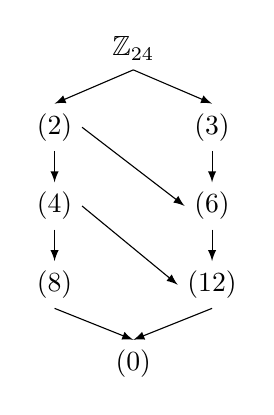
\begin{tikzpicture}
              %\draw[help lines](0,0) grid (6,6);
              \draw (3,5) node[] (n1) {$\mathbb{Z}_{24}$};
              \draw (4,4) node[] (n3) {$(3)$};
              \draw (4,3) node[] (n6) {$(6)$};
              \draw (4,2) node[] (n12) {$(12)$};
              \draw (2,4) node[] (n2) {$(2)$};
              \draw (2,3) node[] (n4) {$(4)$};
              \draw (2,2) node[] (n8) {$(8)$};
              \draw (3,1) node[] (n0) {$(0)$};

              \draw[-latex] (n1.south)--(n2.north);
              \draw[-latex] (n2.south)--(n4.north);
              \draw[-latex] (n4.south)--(n8.north);
              \draw[-latex] (n8.south)--(n0.north);

              \draw[-latex] (n1.south)--(n3.north);
              \draw[-latex] (n3.south)--(n6.north);
              \draw[-latex] (n6.south)--(n12.north);
              \draw[-latex] (n12.south)--(n0.north);

              \draw[-latex] (n2.east)--(n6.west);
              \draw[-latex] (n4.east)--(n12.west);
            \end{tikzpicture}
          \end{center}


        \end{proof}

      \item Question 19: Use the lattice to help find $N_{D_{16}}(\langle
        s,r^4\rangle)$.
        \begin{proof}
          Since normalizers are subgroups, the normalizer
          $N_{D_{16}}(\langle s,r^4\rangle)$ must be one of the six
          possible subgroups of $D_{16}$ shown in the lattice. \\

          To check if
          a subgroup $H$ of $G$ lies within the normalizer of any subset
          $S\subset G$, we show that it suffices to check that each
          generator $g\in H$ of the subgroup commutes with the set $S$:
          Every element $h$ in $H$ is a finite product its generators.
          In other words, $h=g_1\cdots g_n$ for some generators
          $g_i\in H$, and $n\in\mathbb{N}$. It suffices to show by
          induction on $n$ that $g_1\cdots g_n$ commutes with $S$ if all
          generators commute with $S$. The base case where $n=1$ is true by
          assumption. For step $n+1$, we have
          \begin{align*}
            g_1\cdots g_{n+1}S  &= (g_1\cdots g_n)g_{n+1}S  & \\
                                &= (g_1\cdots g_n)Sg_{n+1}  & (\text{Base
                                case}) \\
                                &= S(g_1\cdots g_n)g_{n+1}  &
                                (\text{Inductive step}) \\
                                &= Sg_1\cdots g_{n+1},      & \\
          \end{align*}
          which concludes our proof that $H$ lies in $N_G(S)$ as long as
          each of its generators $g_i$ lie in $N_G(S)$. \\

          Next, we show that to check if an element $g\in G$ lies in the
          normalizer of a subgroup $H$ of $G$, where $H$ is generated by
          generators $\{h_i\}_{i\in I}$, it suffices to check that the
          conjugation of each generator $h_i$ under $g$ lies in $H$.
          Given any element $h$ in $H$, $h=h_1\cdots h_n$ for some
          generators $h_i\in H$. Like what we have proven above, we show by
          induction on $n$ that if $gh_ig^{-1}\in H$ for each generator
          $h_i$, then $g(h_1\cdots h_n)g^{-1}$ would also lie in $H$. The
          base case where $n=1$ is true by assumption. For step $n+1$, we
          have
          \begin{align*}
            g(h_1\cdots h_{n+1})g^{-1}  &= (g(h_1\cdots
                                        h_n)g^{-1})(gh_{n+1}g^{-1}), \\
          \end{align*}
          which lies in $H$ since $g(h_1\cdots h_n)g^{-1}$ lies in $H$ by
          induction hypothesis and $gh_{n+1}g^{-1}$ lies in $H$ by base
          case. \\

          Summarizing our two arguments above, to check if a subgroup of
          $D_{16}$ lies in the normalizer of $H=\langle s,r^4\rangle$, it
          suffices to check that each generator of $H$ under conjugation by
          any generator of the subgroup remains in $H$. We go through
          the generators of each subgroup of $D_{16}$ to identify the
          largest subgroup $K$ whose generators all commute with $H$. That
          subgroup $K$ would be the normalizer of $H$. \\

          Now after the multiplying out the generators of $H$ and using the
          rules $s^2=r^8=1$ and $rs=sr^{-1}$ of $D_{16}$, we find that $H$
          contains four unique elements: $H=\{1,s,r^4,sr^4\}$. We find that
          $D_{16}$'s largest non-trivial subgroup $\langle s,r^2\rangle$
          lies in the normalizer of $H$ because the generators $s$ and $r^4$
          of $H$, under conjugation by $s$ or $r^2$, remain in $H$.
          However, $D_{16}$ does not lie in the normalizer because
          element $r$ of $D_{16}$ does not commute with $H$. More
          specifically, $rsr^{-1}=sr^{-2}=sr^6$, which does not lie in $H$,
          because in $D_{16}$, elements $s^{a_1}r^{b_1}$ and
          $s^{a_2}r^{b_2}$ are equal if and only if $a_1\equiv a_2\pmod{2}$
          and $b_1\equiv b_2\pmod{8}$. Hence, the normalizer of $\langle
          s,r^4\rangle$ is $\langle s,r^2\rangle$.
        \end{proof}
    \end{enumerate}

  \item Section 3.1
    \begin{enumerate}
      \item Question 25:
        \begin{enumerate}
          \item Prove that a subgroup $N$ of $G$ is normal if and only if
            $gNg^{-1}\subseteq N$ for all $g\in G$.
            \begin{proof}
              The forward implication is true by definiton of a normal
              subgroup. To prove the reverse implication, it suffices to
              show that if $gNg^{-1}\subseteq N$ for all $g\in G$, then
              $gNg^{-1}\supset N$. This is true by setting $g=e$.
            \end{proof}

          \item Let $G=GL_2(\mathbb{Q})$, let $N$ be the subgroup of upper
            triangular matrices with integer entries and 1's on the
            diagonal, and let $g$ be the diagonal matrix with entries 2,1.
            Show that $gNg^{-1}\subseteq N$ but $g$ does not normalize $N$.

            \begin{proof}
              Given
              \begin{align*}
                n = 
                \begin{array}{*{2}c}
                  1 & i \\
                  0 & 1 \\
                \end{array}
                \in N,
              \end{align*}
              we get
              \begin{align*}
                gng^{-1} & = 
                \begin{array}{*{2}c}
                  2 & 0 \\
                  0 & 1 \\
                \end{array}
                \begin{array}{*{2}c}
                  1 & i \\
                  0 & 1 \\
                \end{array}
                \begin{array}{*{2}c}
                  0.5 & 0 \\
                  0 & 1 \\
                \end{array} \\
                & =
                \begin{array}{*{2}c}
                  1 & 2i \\
                  0 & 1 \\
                \end{array}
                \in N. \\
              \end{align*}
              Hence $gNg^{-1}\subseteq N$. However, $g$ does not normalize
              $N$ because $gNg^{-1}$ does not contain elements of $N$ with
              top right entries that are odd.
            \end{proof}
        \end{enumerate}

      \item Question 34: Let $D_{2n}=\{r,s\,|\; r^n=s^2=1,rs=sr^{-1}\}$ be
        the usual presentation of the dihedral group of order $2n$ and let
        $k$ be a positive integer dividing $n$.

        \begin{enumerate}
          \item Prove that $N=\langle r^k\rangle$ is a normal subgroup of
            $D_{2n}$.
            \begin{proof}
              From question 34, it suffices to show that $gNg^{-1}\subseteq
              D_{2n}$ for every $g\in D_{2n}$. In our argument for question
              19 of section 2.5, we proved that it suffices to show
              that the generator $r^k$ of $N$ remains in $N$ after
              conjugation with any of the generators $r$ and $s$ of
              $D_{2n}$. Now
              \begin{align*}
                rr^kr^{-1}  &= r^k\in N, \\
              \end{align*}
              and
              \begin{align*}
                sr^ks^{-1}  &= sr^ks    & (\because s^{-1}=s) \\
                            &= ssr^{-k} & (\text{from induction on $k$ and
                            using $rs=sr^{-1}$, can show $rs^k=sr^{-k}$}) \\
                            &= r^{-k}   & (\because s^2=1) \\
                            &\in N,     & \\
              \end{align*}
              which completes our proof.
            \end{proof}

          \item Prove that $D_{2n}/\langle r^k\rangle\cong D_{2k}$.
            \begin{proof}
              Recall $D_{2m}$ has $2m$ distinct elements
              $1,r,\ldots,r^{m-1},s,sr,\ldots,sr^{m-1}$. Hence
              $r^{i_1}s^{j_1}$ equals to $r^{i_2}s^{j_2}$ in $D_{2m}$ if
              and only if $i_1\equiv i_2 \pmod{2}$ and $j_1\equiv
              j_2\pmod{m}$. Consider the map $\phi:D_{2n}/\langle
              r^k\rangle\rightarrow D_{2k}$, defined by $[s^ir^j]\mapsto
              s^ir^{j\mod k}$. We show that this map is an isomorphism. \\

              First, we show that this map is well-defined. If
              $s^{i_1}r^{j_1}$ and $s^{i_2}r^{j_2}$ in $D_{2n}$ belong to
              the same equivalence class, then
              $s^{i_2}r^{j_2}=s^{i_1}r^{j_1}r^{ak}$ for some
              $a\in\mathbb{Z}$. Then from our observation above, this
              implies that $i_1\equiv i_2 \pmod{2}$ and $j_1\equiv
              j_2+ak\pmod{n}$. Then since $k$ divides $n$, this means
              $j_1\equiv j_2\pmod{k}$, which implies that $s^{i_1}r^{j_1}$
              and $s^{i_2}r^{j_2}$ will be mapped to the same element
              $s^{i_1}r^{j_1\mod{k}}$ in $D_{2k}$. Hence the map $\phi$ is
              well-defined. \\

              Next, we show that $\phi$ is a homomorphism. It is routine to
              show that $\phi([s][s])=\phi([s])\phi([s])$ and
              $\phi([r][r])=\phi([r])\phi([r])$. Also,
              \begin{align*}
                \phi([s][r])  &= \phi([sr])           & (\because
                [a][b]=[ab]\; \text{for quotient maps})\\
                              &= sr^{1\mod{k}}        & \\
                              &= sr                   & \\
                              &= \phi([s])\phi([r]),  & \\
              \end{align*}
              and
              \begin{align*}
                \phi([r][s])  &= \phi([rs])       & (\because [a][b]=[ab]\;
                \text{for quotient maps}) \\
                              &= \phi(sr^{n-1})   & \\
                              &= sr^{n-1\mod{k}}  & \\
                              &= sr^{-1\mod{k}}   & (\because k|n) \\
                              &= sr^{k-1}         & \\
                              &= (r^{k-1})^{-1}s  & (\text{from induction on
                              $k$ and using $rs=sr^{-1}$, can show
                              $rs^k=sr^{-k}$}) \\
                              &= rs               & \\
                              &= \phi([r])\phi([s]).  \\
              \end{align*}
              Since $D_{2n}$ is generated by $r$ and $s$, given any
              $x,y\in D_{2n}$, we can express $x$ and $y$ as a finite
              sequence of $r$'s and $s$'s. Then from induction on the
              length of the sequences, and using the above rules, where
              $\phi([s][s])=\phi([s])\phi([s])$,
              $\phi([r][r])=\phi([r])\phi([r])$,
              $\phi([r][s])=\phi([r])\phi([s])$,
              $\phi([s][r])=\phi([s])\phi([r])$, we can
              show that $\phi([x][y])=\phi([x])\phi([y])$. Hence $\phi$ is
              a homomorphism. \\

              $\phi$ is surjective since every $sr^i\in D_{2k}$ has an
              inverse $sr^i$ in $D_{2n}$. It remains to show that $\phi$
              is injective. This is equivalent to showing that the kernel
              of $\phi$ contains only the identity $[1]$.
              In $D_{2k}$, two elements $r^{i_1}s^{j_1}$ and
              $r^{i_2}s^{j_2}$ are equal if and only if $i_1\equiv i_2
              \pmod{2}$ and $j_1\equiv j_2\pmod{k}$. Hence the inverse
              image of $\phi$ on $1=s^0r^0\in D_{2k}$ can only be of the
              form $[r^{4i}]$, where $i\in\mathbb{Z}$. Since
              $[r^{4i}]=[1]$, the kernel contains only the identity. So
              $\phi$ is an isomorphism, which completes our proof that the
              two groups are isomorphic.
            \end{proof}
        \end{enumerate}

      \item Question 35: Prove that $SL_n(F)\unlhd GL_n(F)$ and describe
        the isomorphism type of the quotient group.
        \begin{proof}
          To prove a subgroup $N$ of $G$ is normal, it suffices to show
          that $gNg^{-1}\subseteq G$ for every $g\in G$. Given $g\in
          GL_n(F)$ and $h\in SL_n(F)$,
          \begin{align*}
            |ghg^{-1}|  &= |g||h||g^{-1}| \\
                        &= |g||h|/|g|     \\
                        &= |h|            \\
                        &= 1,             \\
          \end{align*}
          which implies that $ghg^{-1}\in SL_n(F)$. Hence $SL_n(F)\unlhd
          GL_n(F)$. \\

          The quotient group is isomorphic to $(F^*,\times)$. We show that
          the map $\phi$ that sends $[A]$ in the quotient group to $|A|$ is
          an isomorphism. The map is well-defined because $[A]=[B]$ if and
          only if $AB^{-1}\in SL_n(F)$ if and only if $|AB^{-1}|=1$ if and
          only if $|A|=|B|$. The map is homormorphic because
          $\phi([A][B])=\phi([AB])=|AB|=|A||B|=\phi([A])\phi([B])$. The map
          is also surjective since every $f\in F^*$ has an inverse image
          $[fI]$. Finally, the map is injective because the kernel contains
          only identity - $\phi([A])=1$ if and only if $|A|=1$ if and only
          if $A\in SL_n(F)$ if and only if $[A]=[1]$. Hence the quotient
          group is isomorphic to $(F^*,\times)$.
        \end{proof}

      \item Question 36: Prove that if $G/Z(G)$ is cyclic then $G$ is
        abelian.
        \begin{proof}
          Assume $G/Z(G)$ is cyclic. So $G/Z(G)=\langle[x]\rangle$ for some
          $x\in G$. Then given any $g\in G$, $[g]=[x]^a=[x^a]$ for some
          $a\in\mathbb{Z}$, which means $g=x^az$ for some $z\in Z(G)$. \\

          So given $g_1,g_2\in G$, we have $g_1=x^{a_1}z_1$ and
          $g_2=x^{a_2}z_2$ for some $a_1,a_2\in\mathbb{Z}$, $z_1,z_2\in
          Z(G)$. Then
          \begin{align*}
            g_1g_2  &= x^{a_1}z_1x^{a_2}z_2 & \\
                    &= x^{a_1+a_2}z_2z_1    & (\because z_1\,
                    \text{commutes}) \\
                    &= x^{a_2}x^{a_1}z_2z_1 & \\
                    &= x^{a_2}z_2x^{a_1}z_1 & (\because z_2\,
                    \text{commutes}) \\
                    &= g_2g_1,              & \\
          \end{align*}
          so $G$ is abelian.
        \end{proof}
    \end{enumerate}
\end{enumerate}
\end{document}
